\chapter{Область устойчивости}
Рассмотрим систему 3-го порядка, заданную структурной схемой, 
представленной на рисунке 8. Определим, при каких значениях постоянных 
времени \( T_1 \) и \( T_2 \) полюса соответствующих передаточных функций совпадут с
набором корней \( \lambda_{1} = -3,\,\lambda_{2} = -1 \) из Задания 1.
\begin{figure}[H]
    \centering
    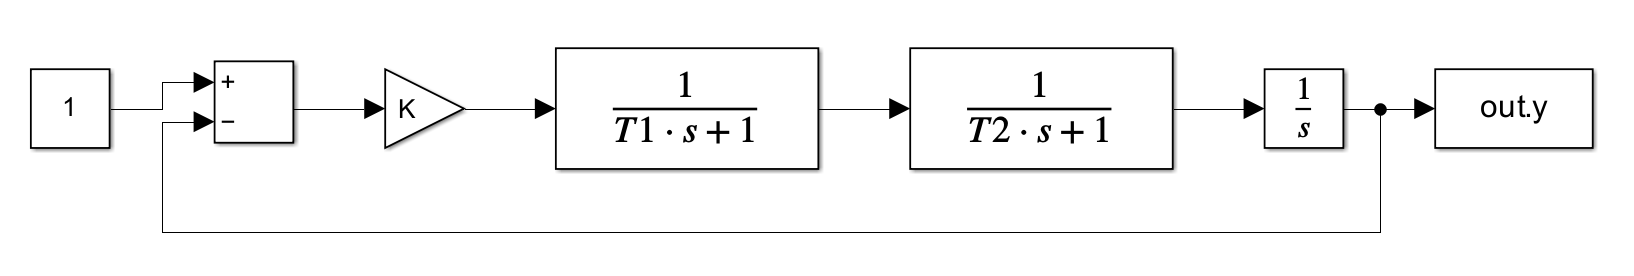
\includegraphics[width=1\textwidth]{../images/sim2.png}
    \caption{Simulink схема системы для задания 2}
\end{figure}

Найдем \( T_1 \) при котором полюса передаточной функции системы совпадают с 
\( \lambda_{1} = -3\). Для этого приравняем ее знаменатель к нулю:
\[
    T_1s + 1 = 0
\]
\[
    T_1\lambda_1 + 1 = 0
\]
\[
    T_1 = \frac{-1}{\lambda_1} = \frac{1}{3}
\]
Аналогично найдем \( T_2 \):
\[
    T_2s + 1 = 0
\]
\[
    T_2\lambda_2 + 1 = 0
\]
\[
    T_2 = \frac{-1}{\lambda_2} = 1
\]
Зафиксируем значение \( T_2 = 1 \) и определим границу устойчивости в 
пространстве параметров \( K \) и \( T_1 \), используя критерий Гурвица. 
Запишем дифференциальное уравнение, соответствующее структурной схеме:
\[
y = \frac{1}{p} \left( \frac{1}{p + 1} \left( \frac{1}{T_1 p + 1} \left( K(g - y) \right) \right) \right)
\]

\[
T_1 \dddot{y} + (1 + T_1) \ddot{y} + \dot y + Ky = Kg
\]

\[
\dddot{y} + \frac{(1 + T_1) \ddot{y}}{T_1}+ \frac{\dot y}{T_1} + \frac{Ky}{T_1} = \frac{Kg}{T_1}
\]

Так как движение свободное:

\[
\dddot{y} + \frac{(1 + T_1) \ddot{y}}{T_1}+ \frac{\dot y}{T_1} + \frac{Ky}{T_1} = 0
\]

Рассмотрим критерий Гурвица при \( K>0 \) и \( T_1>0 \):
\[
a_0 = \frac{K}{T_1}, \, a_1 = \frac{1}{T_1}, \, a_2 = \frac{1 + T_1}{T_1}
\]
\[
\Delta_1 = |a_2| = \frac{1 + T_1}{T_1} > 0
\]
\[
\Delta_2 = \begin{vmatrix}
    a_2 & a_0 \\
    1 & a_1
\end{vmatrix}
= \frac{1 + T_1}{T_1} \cdot \frac{1}{T_1} - \frac{K}{T_1} = \frac{1+T_1}{T_1^2} - \frac{K}{T_1} > 0
\Rightarrow K < \frac{1+T_1}{T_1}
\]
\[
\Delta_3 = \begin{vmatrix}
    a_2 & a_0 & 0 \\
    1 & a_1 & 0 \\
    0 & a_2 & a_0
\end{vmatrix} =
\frac{1 + T_1}{T_1} \cdot \frac{1}{T_1} \cdot \frac{K}{T_1} - \frac{K}{T_1} \cdot \frac{K}{T_1}
= \frac{(1+T_1)K - K^2T_1}{T_1^3} > 0
\]

Так как \( T_1 > 0 \), то \(\Delta_1\) всегда положительно. Так как \( K > 0 \) и \( T_1 > 0 \):
\[
\Delta_3 = \frac{(1+T_1)K - K^2 T_1}{T_1^3} > 0
\]
\[
    (1+T_1)K - K^2 T_1 > 0
\]
\[
    K < \frac{1+T_1}{T_1}
\]

Что эквиваленто условию для $\Delta_2$. Соответственно можно оставить только:
\[
    K > 0
\]
\[
    T_1 > 0
\]
\[
    K < \frac{1+T_1}{T_1}
\]

В Матлабе построим область устойчивости:
\begin{figure}[H]
    \centering
    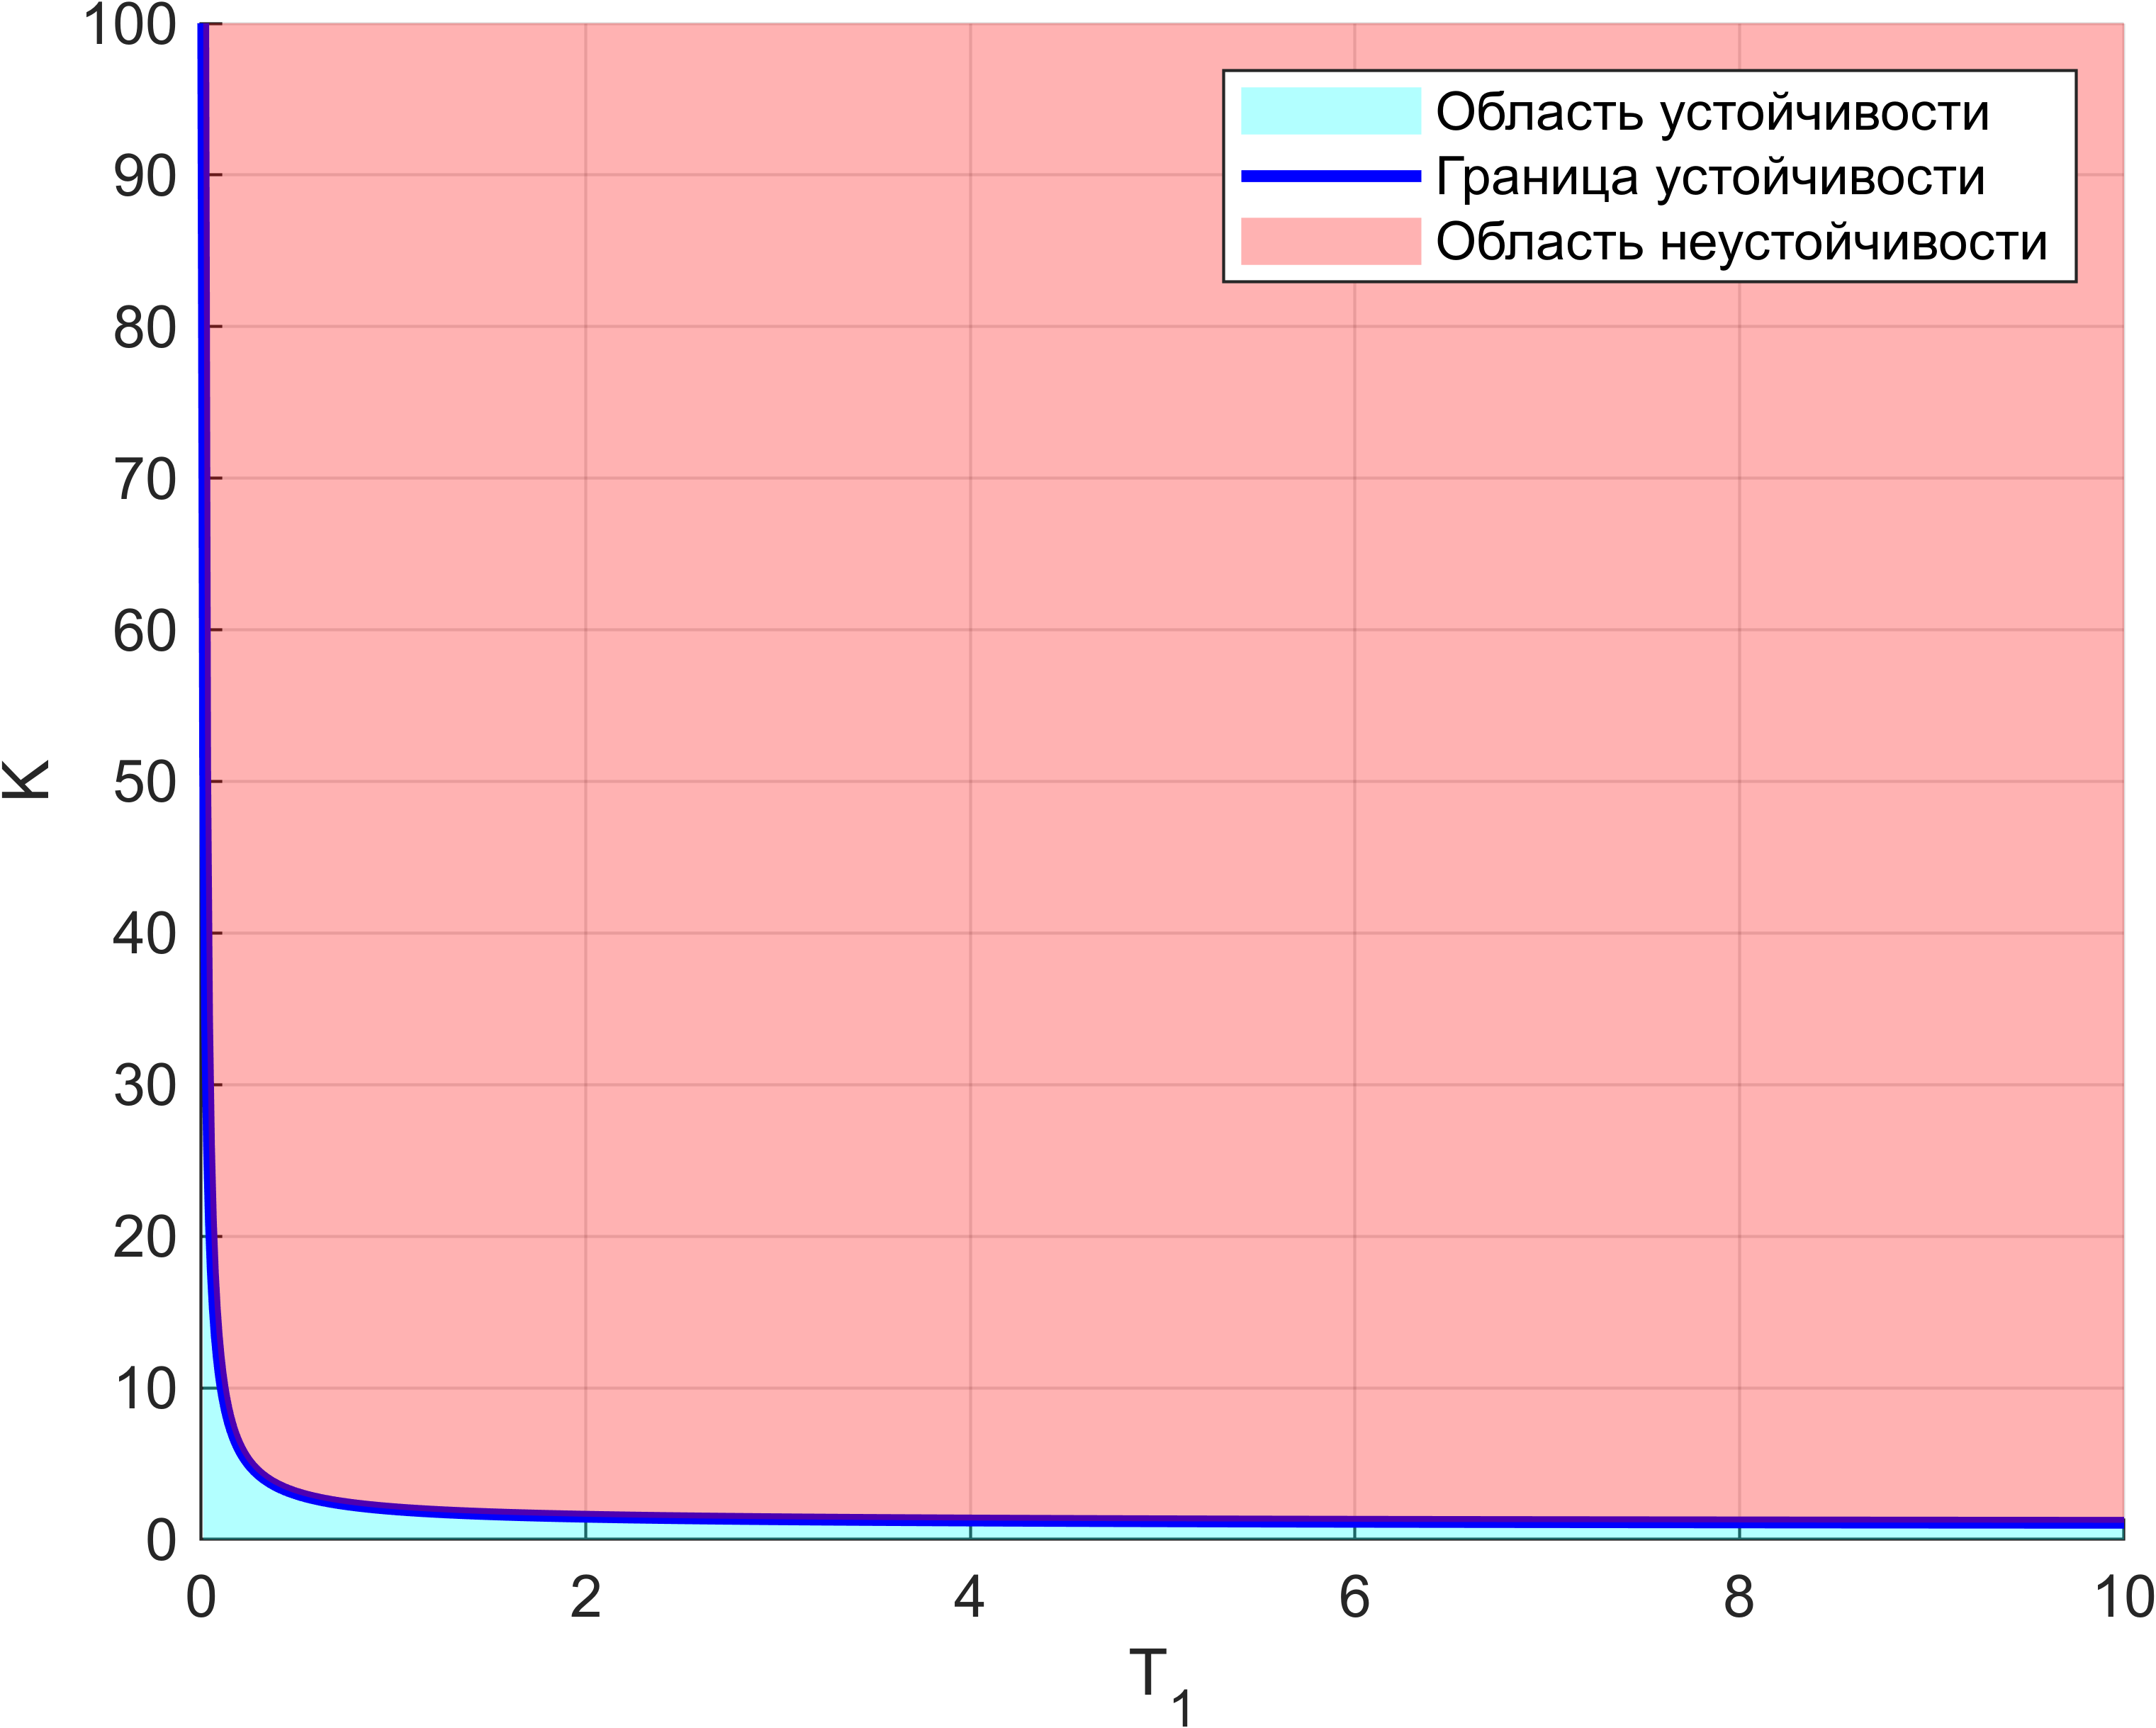
\includegraphics[width=1\textwidth]{../images/2_1.png}
    \caption{Область устойчивости при \( T_2 = const = 1 \)}
\end{figure}

При значениях \( K \) и \( T_1 \) вне области устойчивости система будет неустойчива, 
внутри - асимптотически устойчива.

Теперь найдем границу устойчивости в пространстве параметров \( K \) и \( T_2 \).
дифференциальное уравнение, соответствующее структурной схеме:
\[
y = \frac{1}{p} \left( \frac{1}{T_2p + 1} \left( \frac{1}{\frac{1}{3}p + 1} \left( K(g - y) \right) \right) \right)
\]
\[
\dddot y + \frac{(1 + 3T_2) \ddot y}{T_2} + \frac{3\dot y}{T_2} + \frac{3 K y}{T_2} = \frac{3Kg}{T_2}
\]

Так как движение свободное:

\[
    \dddot y + \frac{(1 + 3T_2) \ddot y}{T_2} + \frac{3\dot y}{T_2} + \frac{3 K y}{T_2} = 0
\]

Рассмотрим критерий Гурвица при \( K>0 \) и \( T_2>0 \):
\[
    a_0 = \frac{3K}{T_2}, \, a_1 = \frac{3}{T_2}, \, a_2 = \frac{1 + 3T_2}{T_2}
\]
\[
\Delta_1 = |a_2| = \frac{1 + 3T_2}{T_2} > 0
\]
\[
\Delta_2 = \begin{vmatrix}
    a_2 & a_0 \\
    1 & a_1
\end{vmatrix}
= \frac{1 + 3T_2}{T_2} \cdot \frac{3}{T_2} - \frac{3K}{T_2} = \frac{3(1+3T_2)}{T_2^2} - \frac{3K}{T_2} > 0
\Rightarrow K < \frac{1+3T_2}{T_2}
\]
\[
\Delta_3 = \begin{vmatrix}
    a_2 & a_0 & 0 \\
    1 & a_1 & 0 \\
    0 & a_2 & a_0
\end{vmatrix} =
\frac{1 + 3T_2}{T_2} \cdot \frac{3}{T_2} \cdot \frac{3K}{T_2} - \frac{3K}{T_2} \cdot \frac{3K}{T_2}
= \frac{9(1+3T_2)K - 9K^2T_2}{T_2^3} > 0
\]

Так как \( T_2 > 0 \), то \(\Delta_1\) всегда положительно. Так как \( K > 0 \) и \( T_2 > 0 \):
\[
\Delta_3 = \frac{9(1+3T_2)K - 9K^2T_2}{T_2^3} > 0
\]
\[
    9(1+3T_2)K - 9 K^2 T_2 > 0
\]
\[
    K < \frac{1+3T_2}{T_2}
\]

Что эквиваленто условию для $\Delta_2$. Соответственно можно оставить только:
\[
    K > 0
\]
\[
    T_2 > 0
\]
\[
    K < \frac{1+3T_2}{T_2}
\]


В Матлабе построим область устойчивости:
\begin{figure}[H]
    \centering
    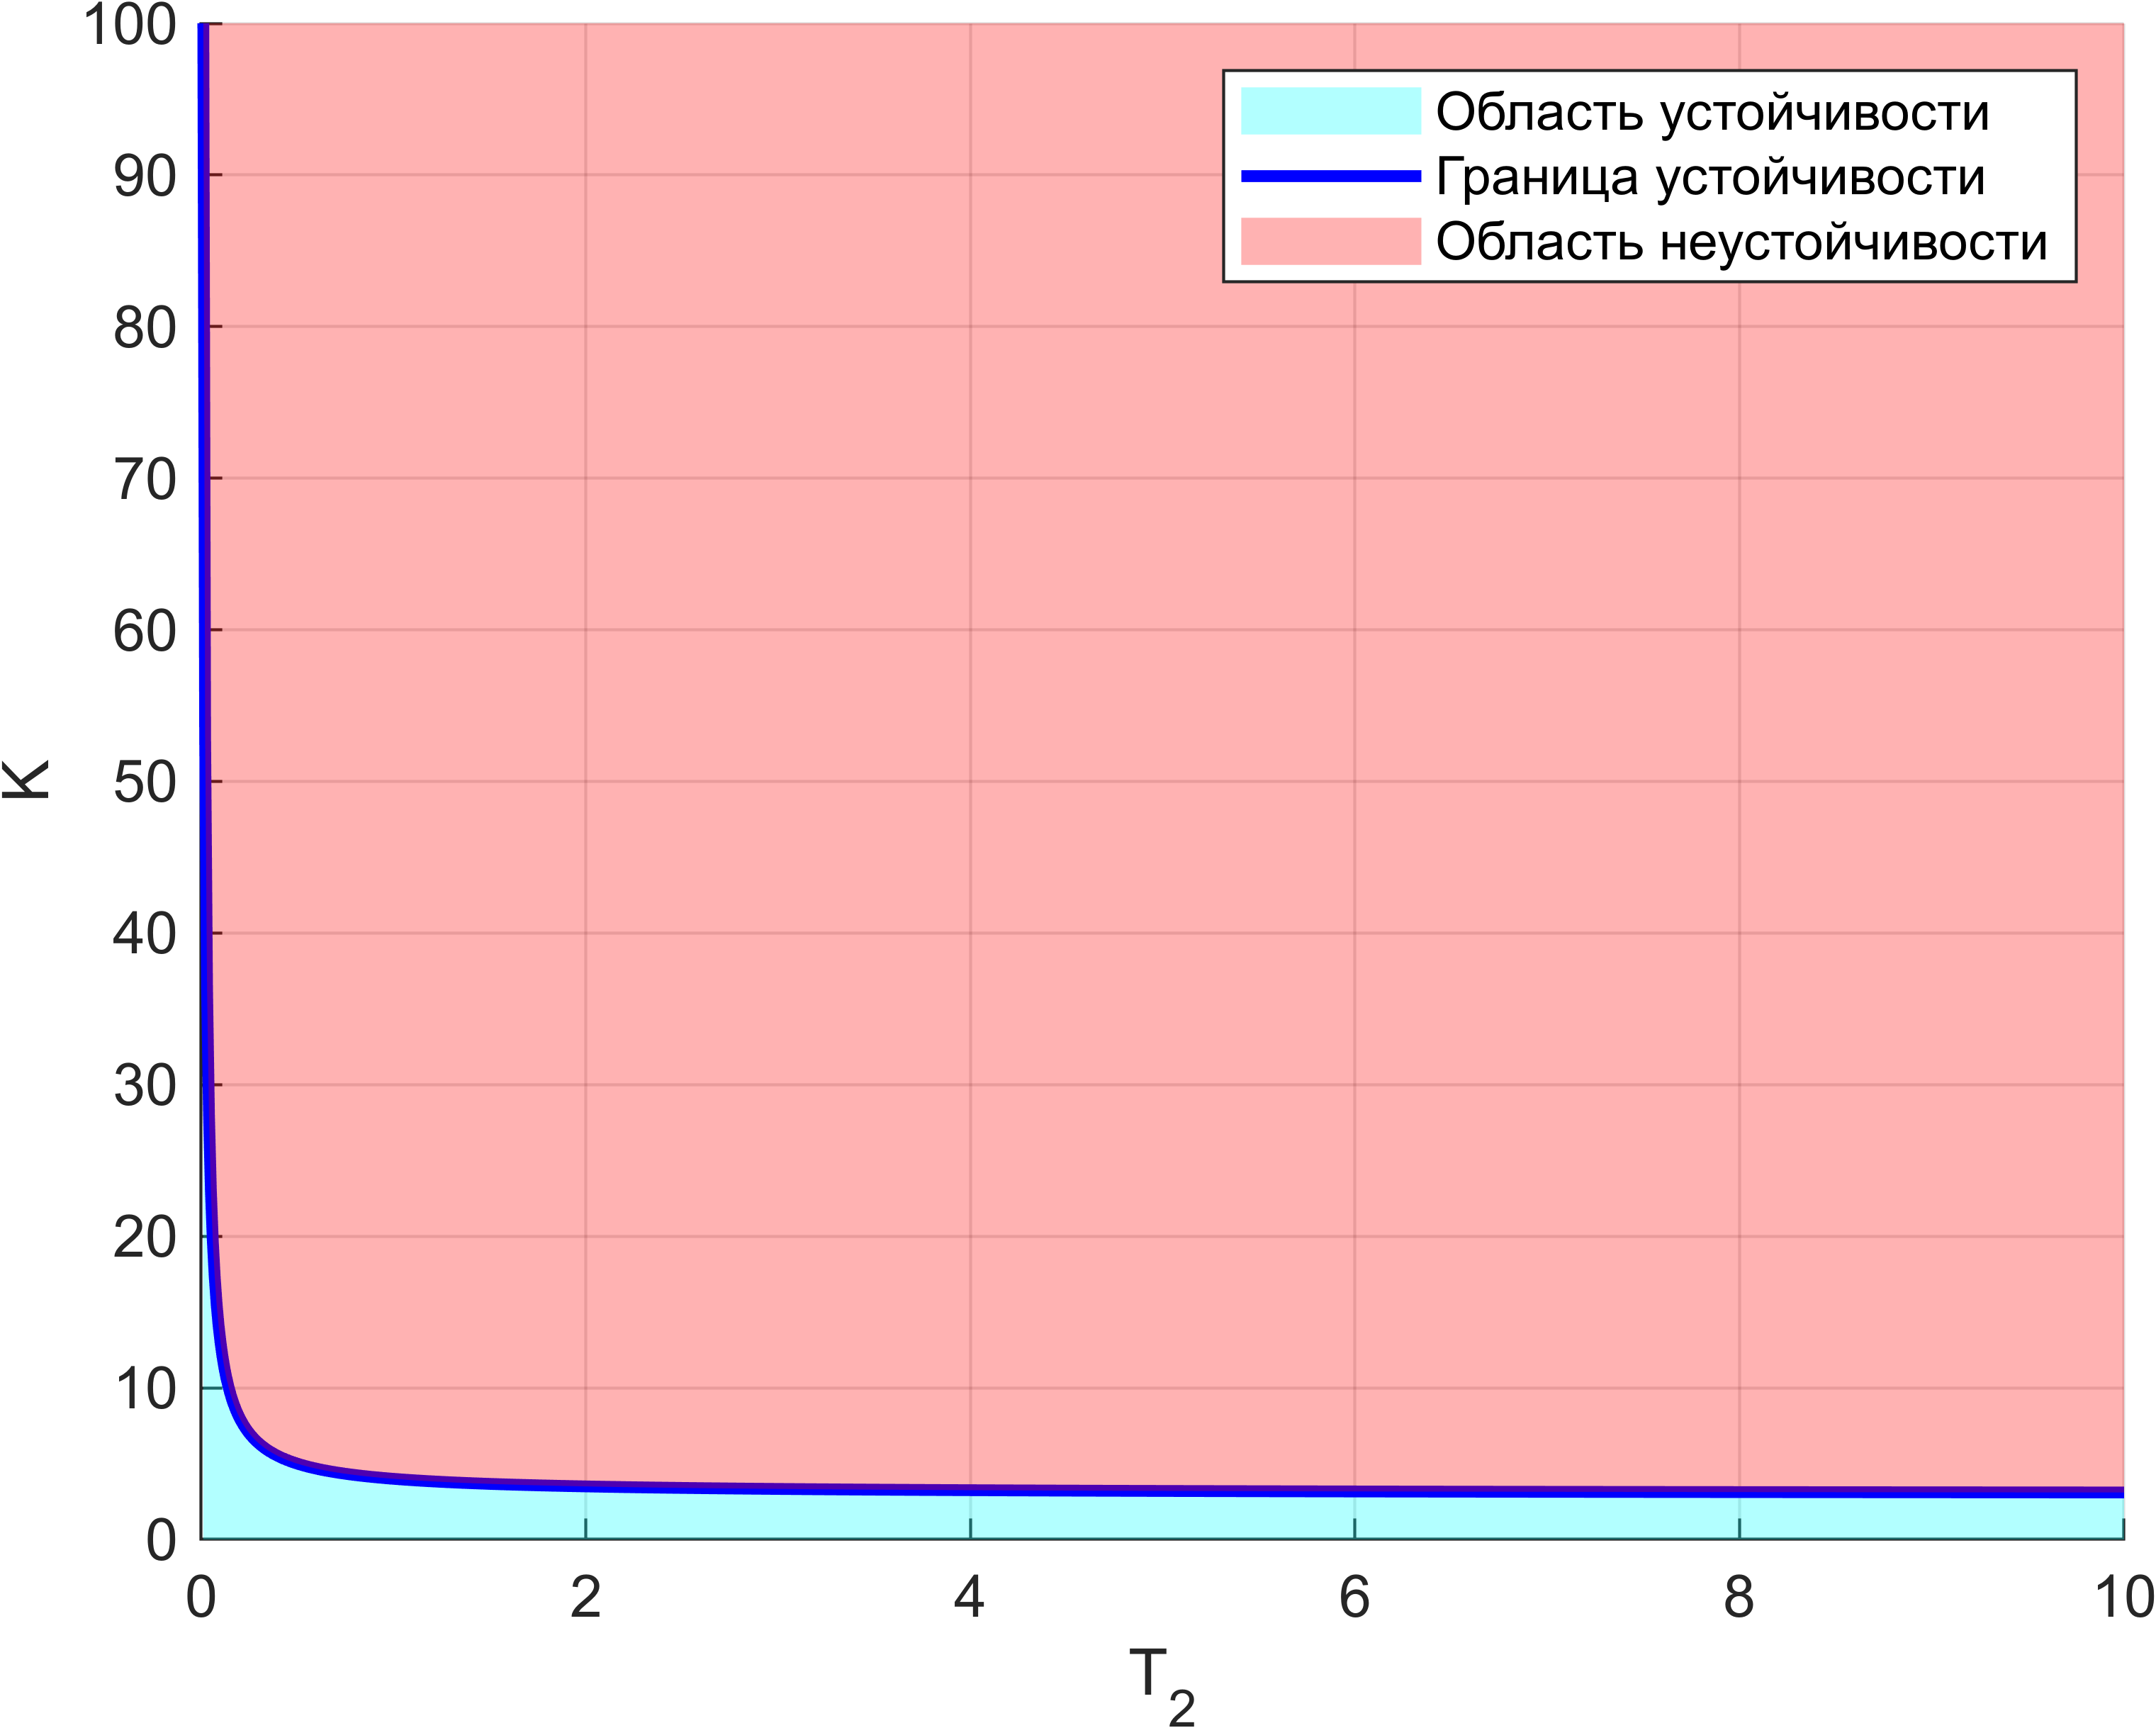
\includegraphics[width=1\textwidth]{../images/2_2.png}
    \caption{Область устойчивости при \( T_1 = const = 1/3 \)}
\end{figure}
\newpage
Исходя из полученных графиков зададим 3 набора параметров \( K \), \( T_1 \), \( T_2 \):

1) Устойчивая система \(K = 1\), \(T_1 = 1\), \(T_2 = 1\):
\begin{figure}[ht]
    \centering
    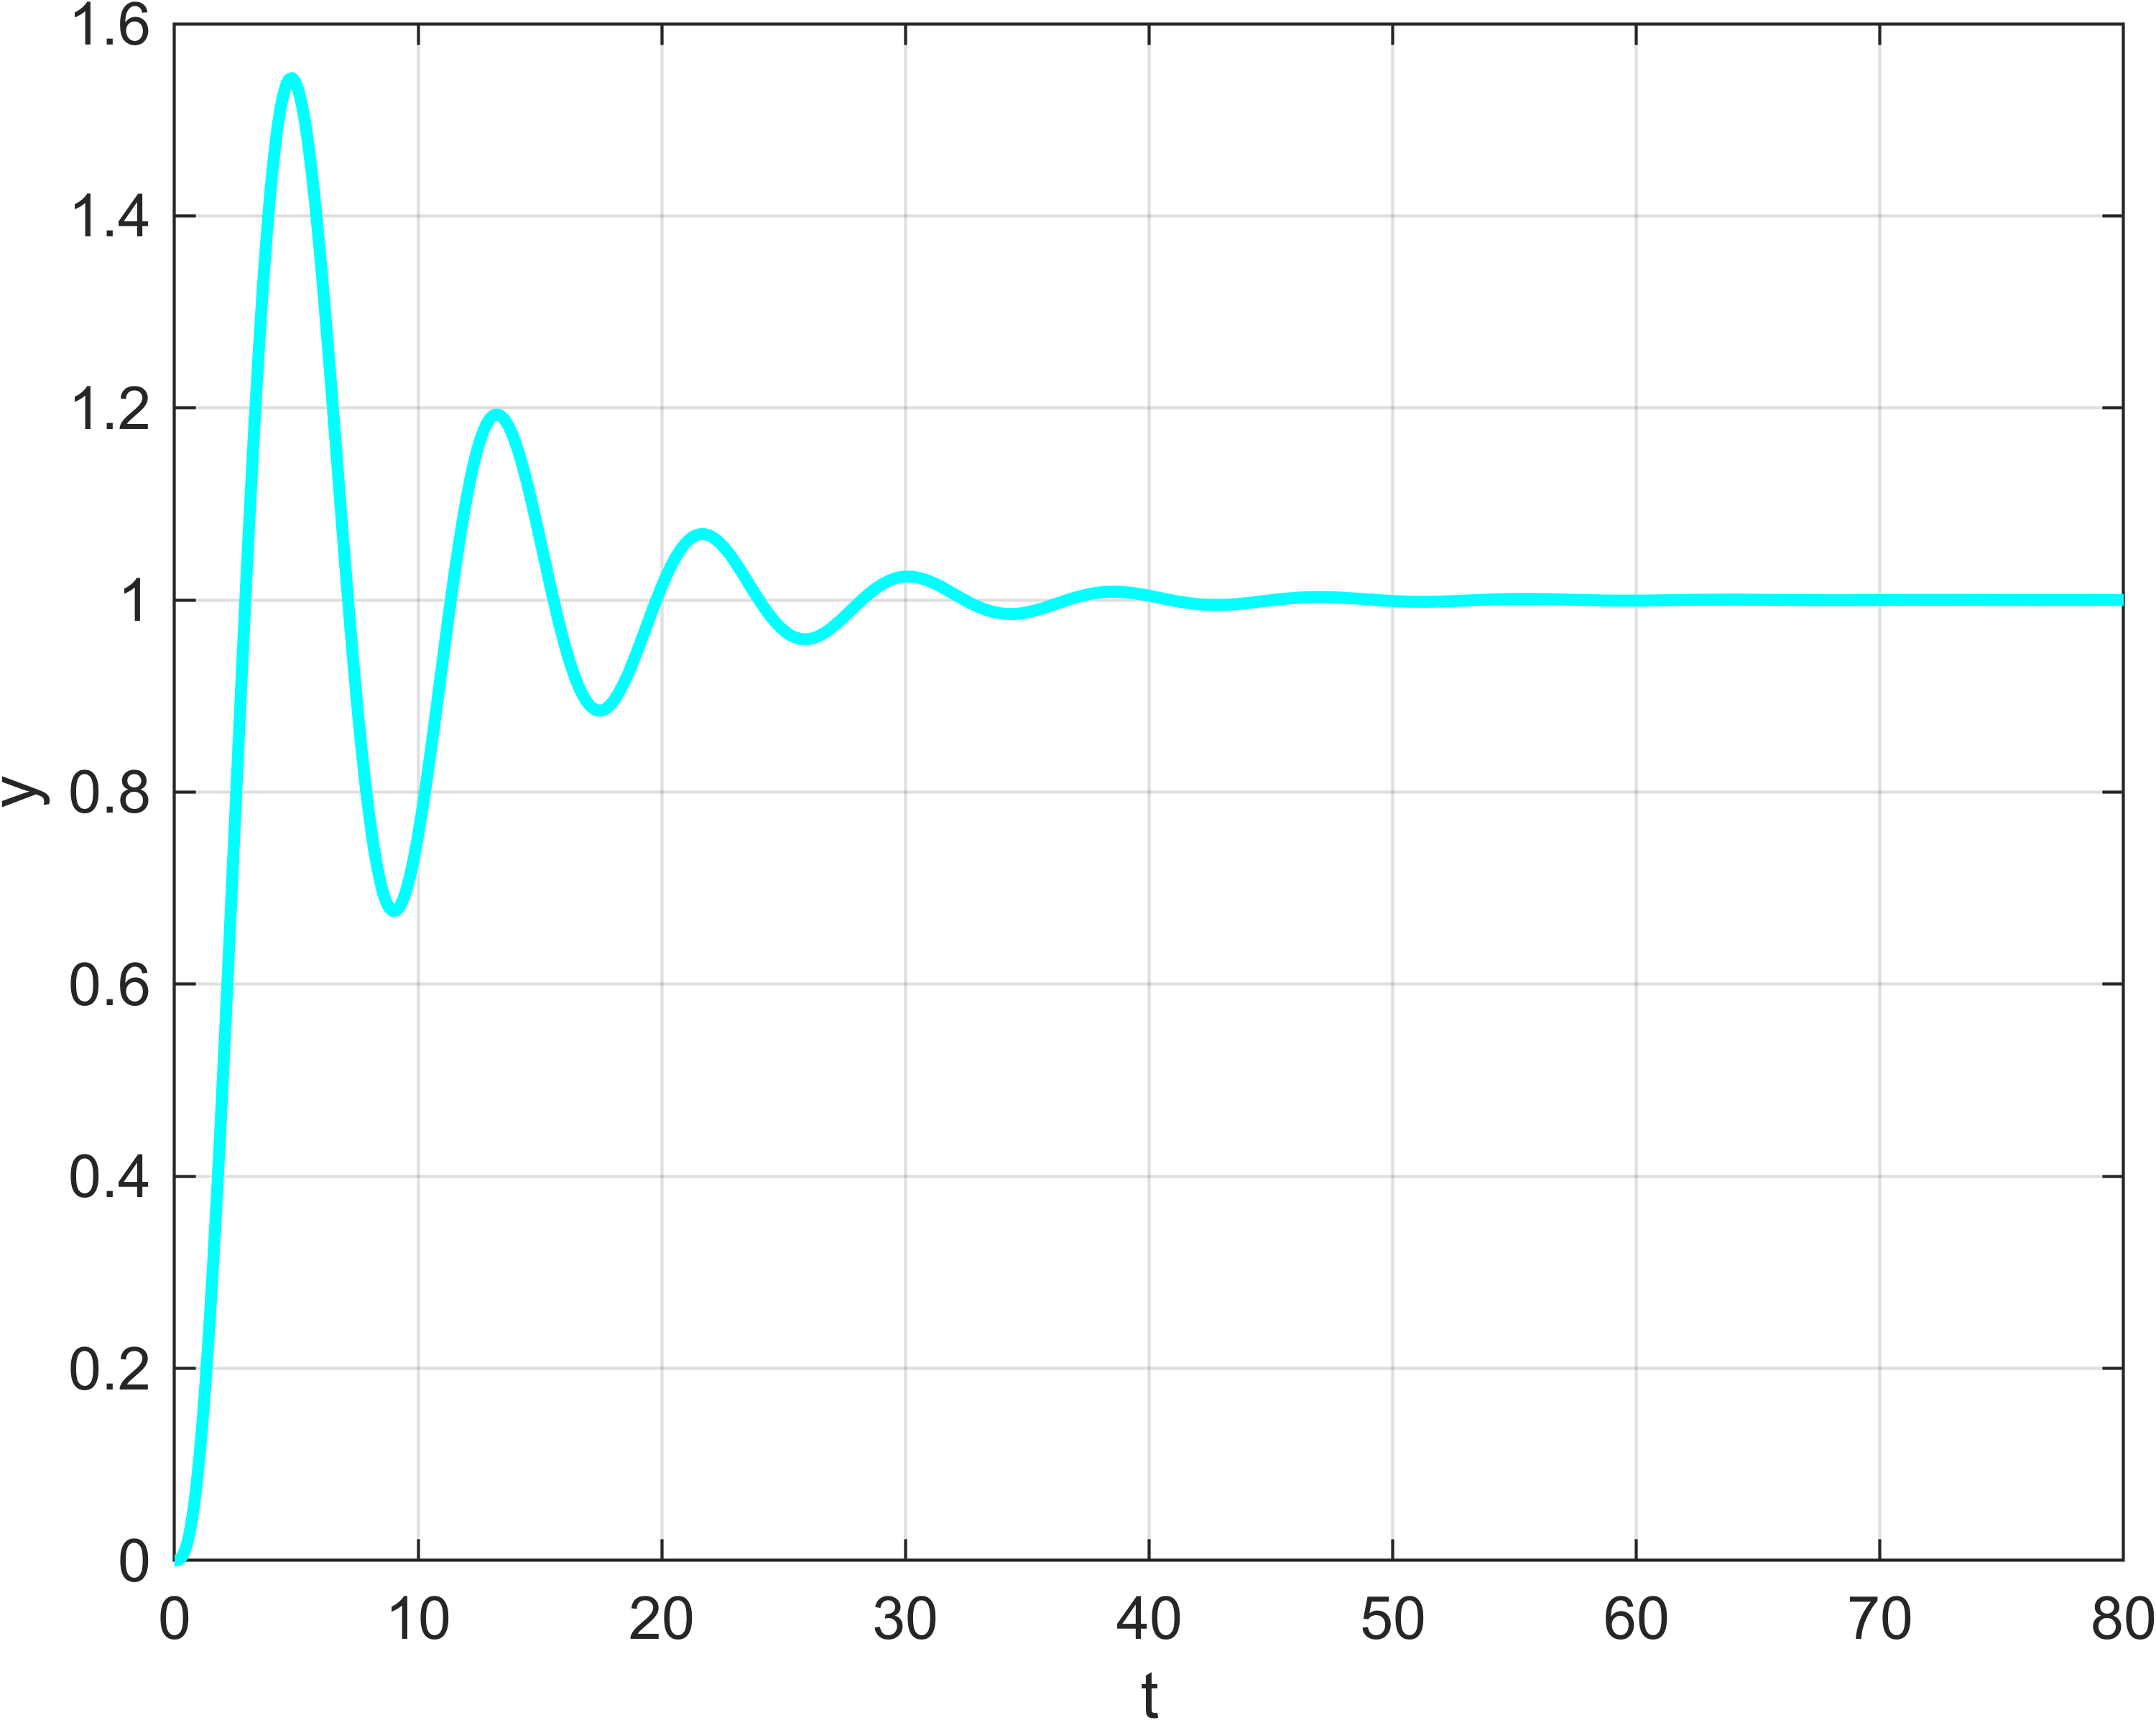
\includegraphics[width=0.7\textwidth, trim={0cm 0cm 0cm 0cm}]{../images/2_3}
    \caption{Устойчивая система}
\end{figure}
% \newpage

2) Неустойчивая система \(K = 2\), \(T_1 = 2\), \(T_2 = 2\):
\begin{figure}[ht]
    \centering
    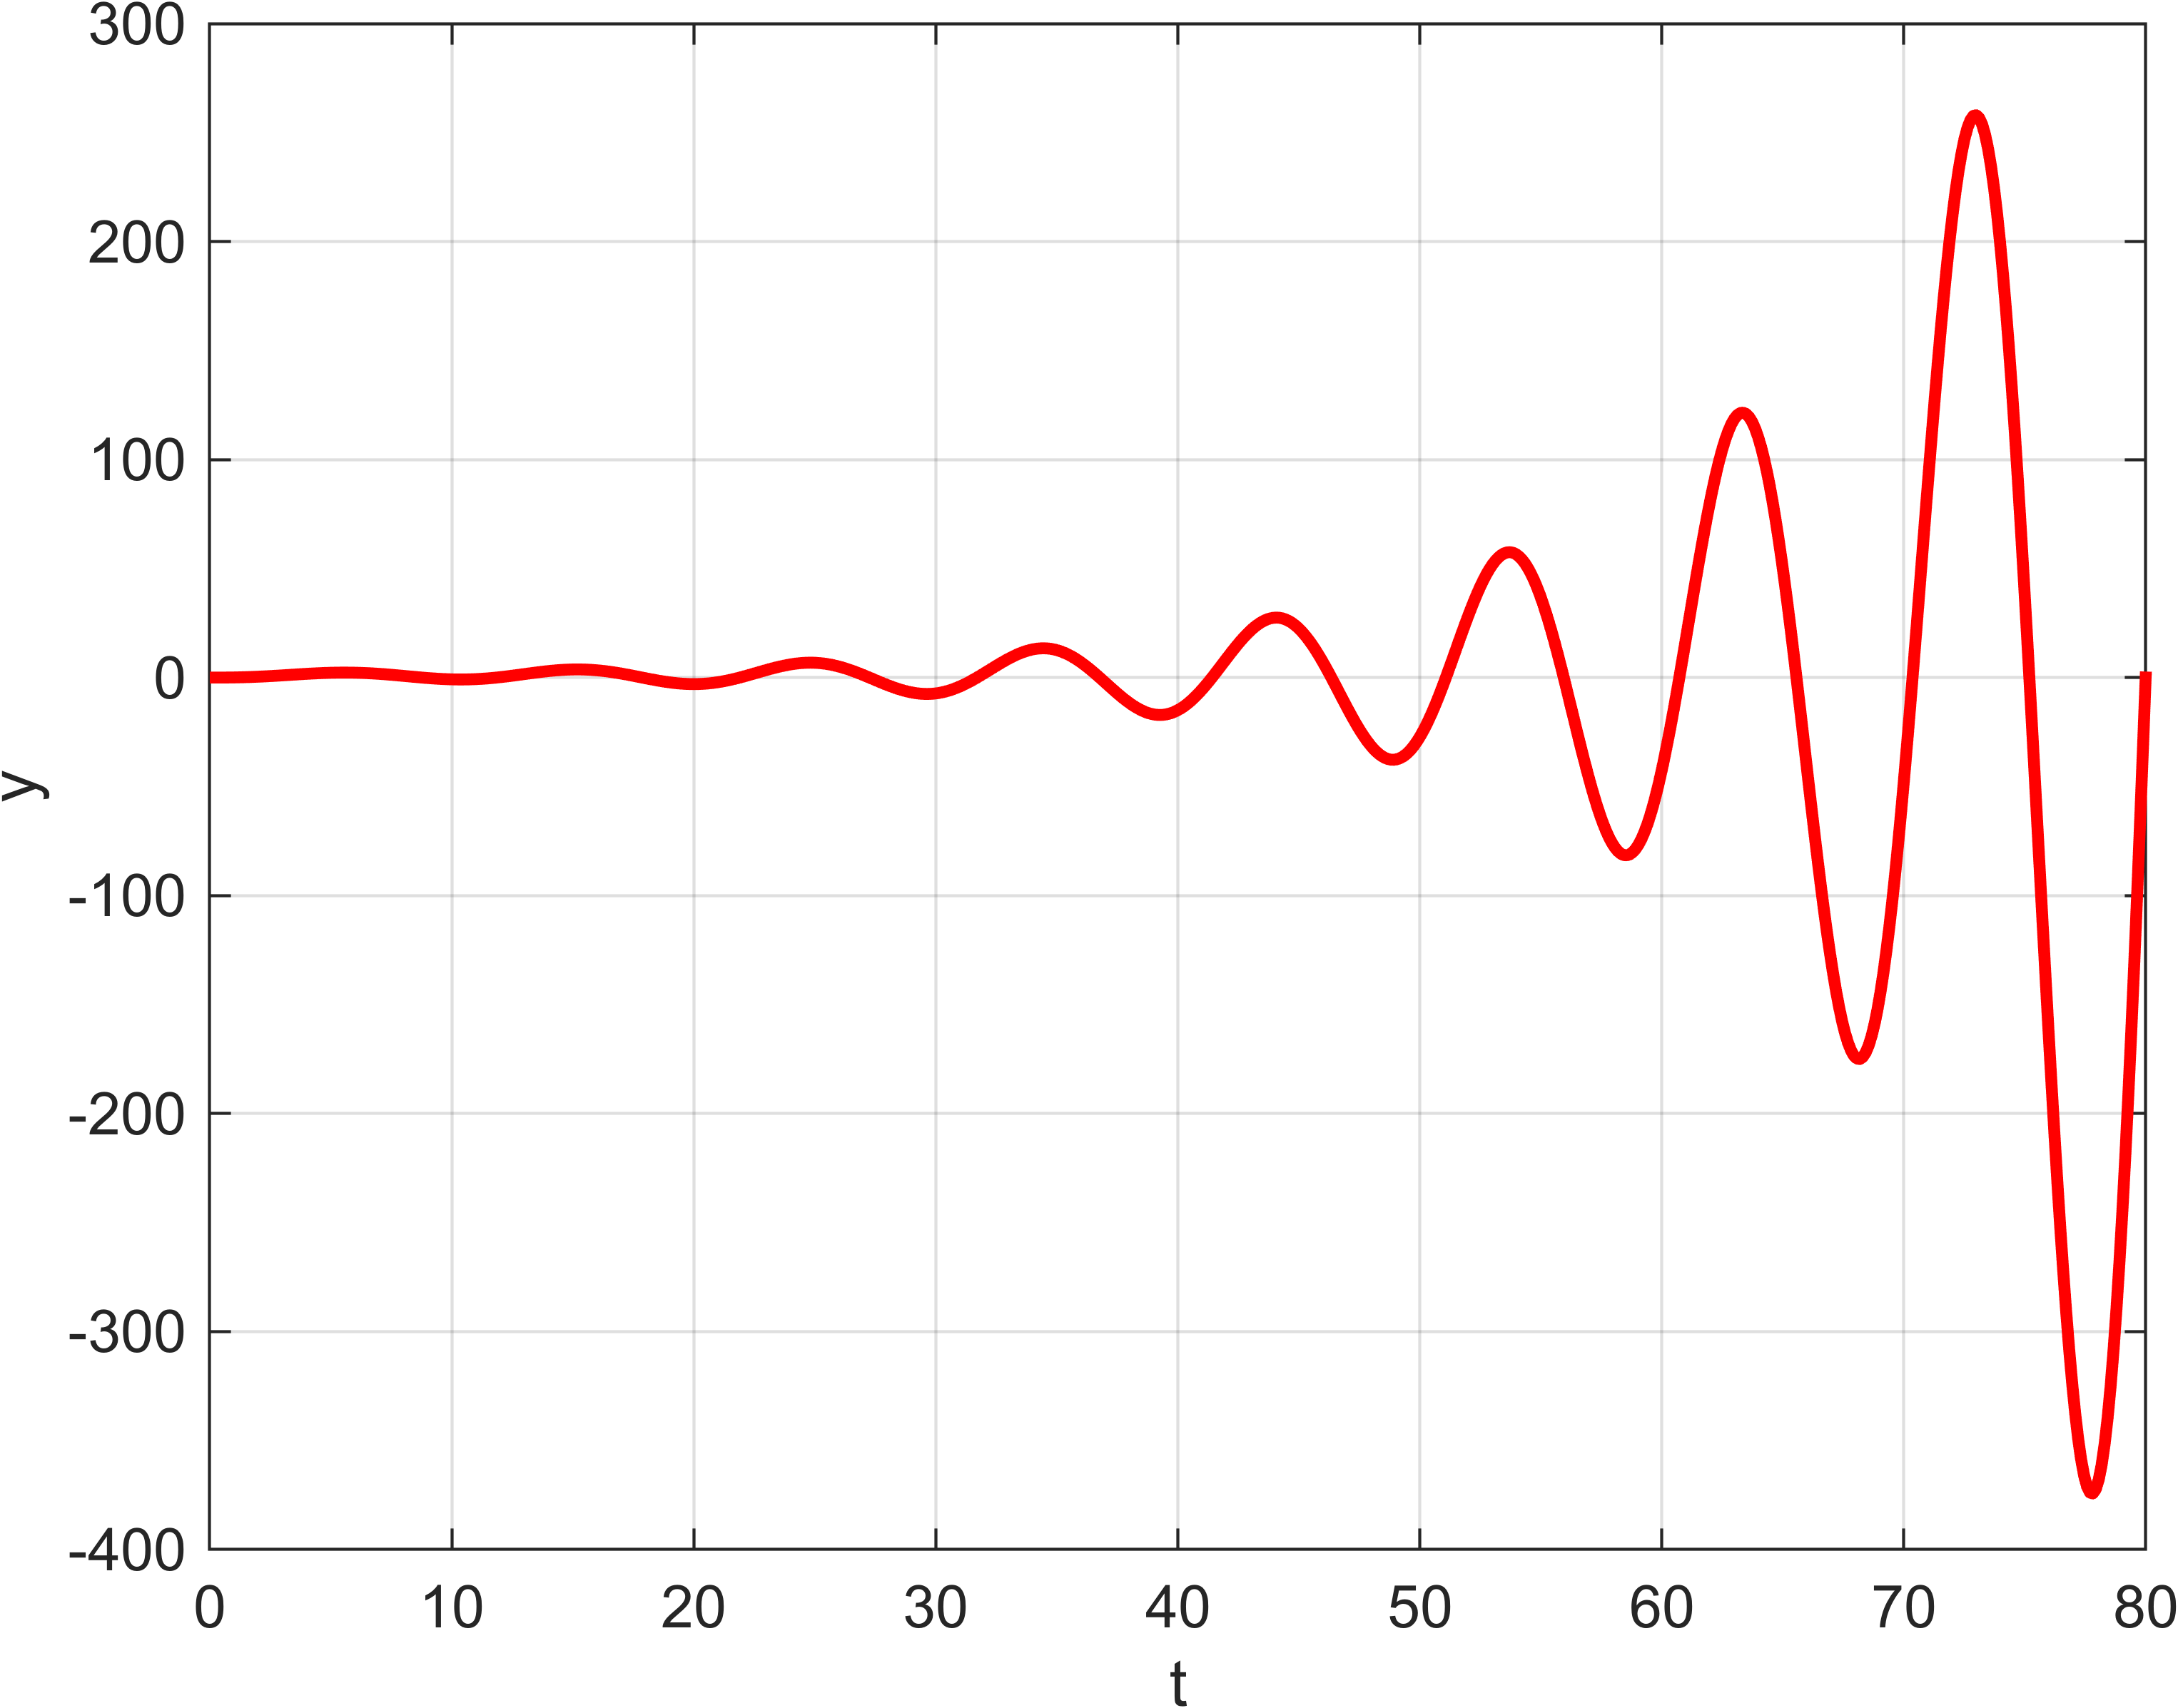
\includegraphics[width=0.7\textwidth, trim={0cm 0cm 0cm 0cm}]{../images/2_4}
    \caption{Неустойчивая система}
\end{figure}
\newpage
3) Система на границе устойчивости \(K = 1\), \(T_1 = 1\), \(T_2 = 2\):
\begin{figure}[ht]
    \centering
    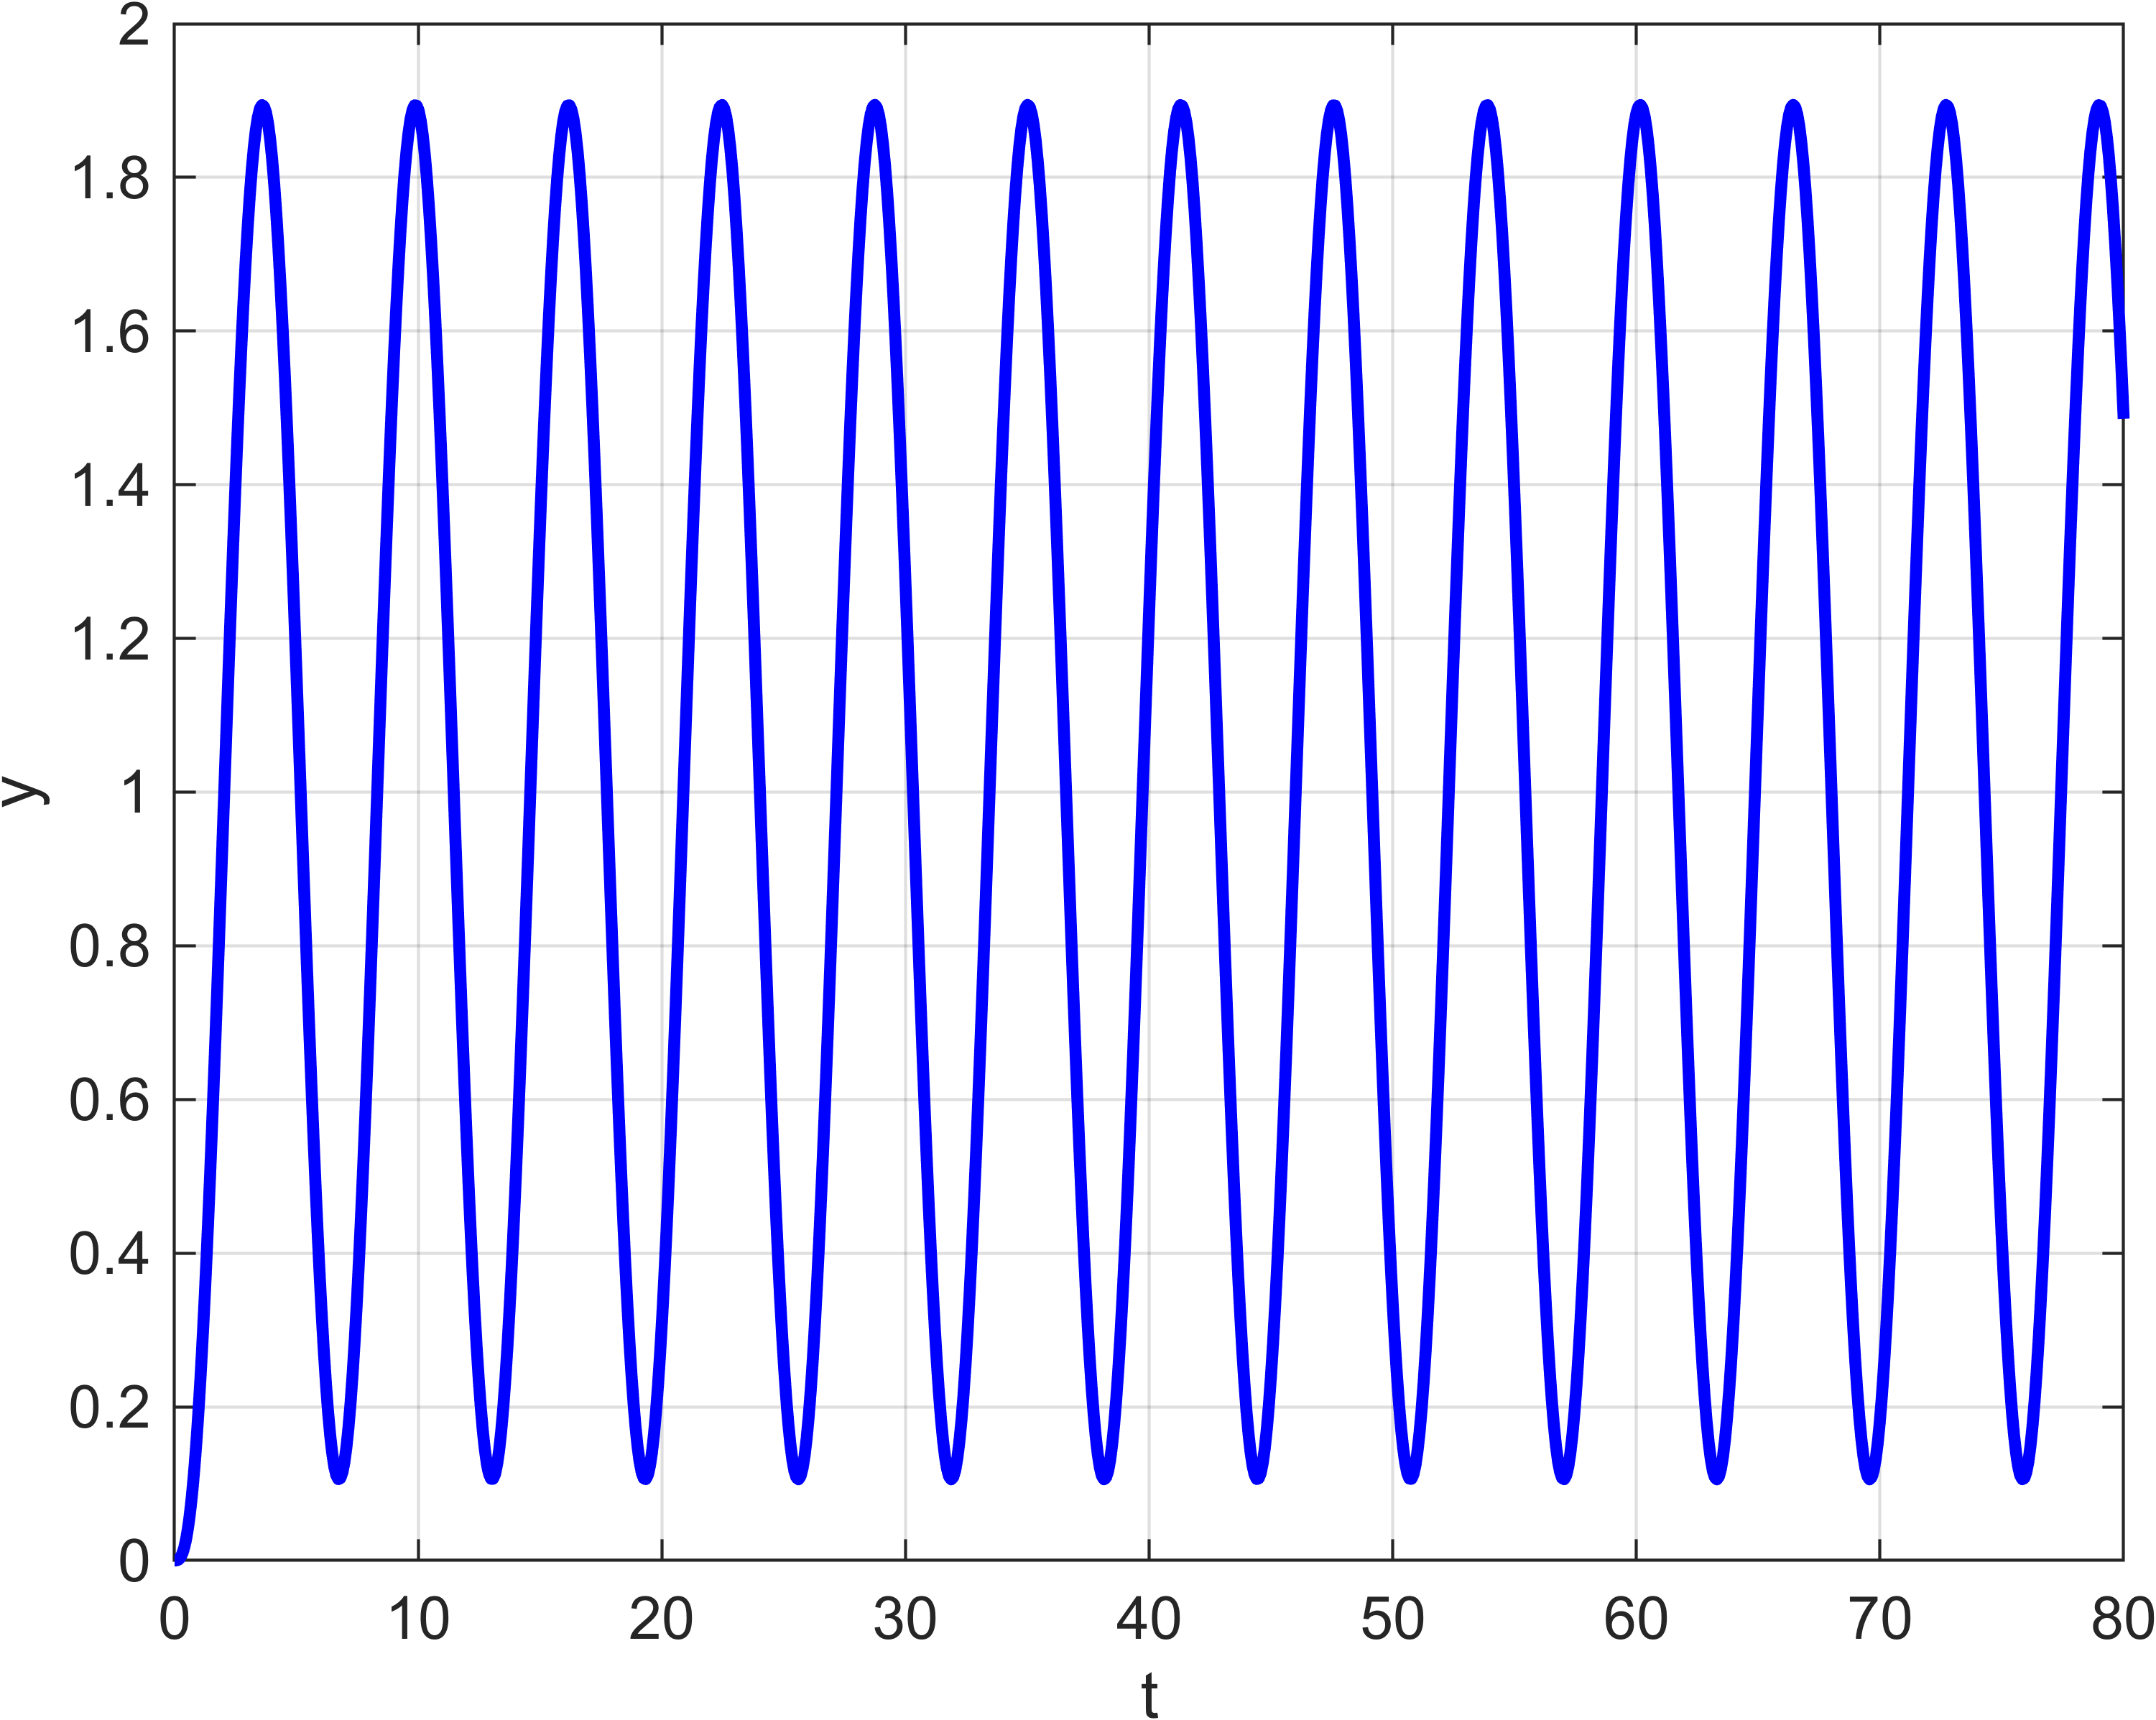
\includegraphics[width=0.7\textwidth, trim={0cm 0cm 0cm 0cm}]{../images/2_5}
    \caption{Система на границе устойчивости}
\end{figure}
\endinput